\documentclass[14pt,a4paper]{extreport}
\usepackage[top=2cm, left=3cm, bottom=2cm, right=1cm]{geometry}
\usepackage[utf8x]{inputenc} % Включаем поддержку UTF8
\usepackage[russian]{babel} % Пакет поддержки русского языка
\usepackage{lscape}
\usepackage{fancyhdr}
\usepackage{textcase}
\graphicspath{{pictures/}}
\DeclareGraphicsExtensions{.pdf,.png,.jpg}
\usepackage{caption}
\usepackage{graphicx}

\title{}
\author{}

\begin{document}
%----------ТИТУЛЬНЫЙ-ЛИСТ--------------
	\center
	Министерство образования Республики Беларусь\\
	Учреждение образования «Белорусский государственный университет информатики и радиоэлектроники»
	\vspace*{2cm}
	\endcenter
	\raggedright
	Факультет компьютерных систем и сетей\\
	\medskip
	Кафедра программного обеспечения информационных технологий\\
	\medskip
	Дисциплина:  Компьютерные системы и сети (КСиС)
	\vspace*{2cm}
	\center
	ПОЯСНИТЕЛЬНАЯ ЗАПИСКА\\
	к курсовому проекту\\
	на тему\\
	\medskip
	Исскуственная нейронная сеть\\
	\medskip
	БГУИР КП  1-40 01 0 116 ПЗ
	\vspace*{4cm}
	\endcenter
	\raggedright
	\hspace*{7.94cm} Студент: гр. 351001 Мельников А.В.\\
	\bigskip
	\hspace*{7.94cm}Руководитель: асс. Третьяков Ф.И.\\
	\center
	\vspace*{6cm}
	Минск 2015
	\pagestyle{empty}
%-------ЛИСТ-ЗАДАНИЯ--------------
	\newpage
	\center
	Учреждение образования\\
	\medskip
	«Белорусский государственный университет информатики и радиоэлектроники»\\
	\medskip
	Факультет компьютерных систем и сетей\\
	\medskip
	\endcenter
	\raggedright
	\hspace*{9.53cm}УТВЕРЖДАЮ\\
	\hspace*{9.53cm}Заведующий кафедрой ПОИТ\\
	\hspace*{9.53cm}\underline{\hspace{6cm}} \\
	\hspace*{11cm}\small (подпись) \normalsize\\
	\hspace*{9.53cm}\underline{\hspace{5cm}}2015 г.\\
	\medskip
	\center
	ЗАДАНИЕ\\
	по курсовому проектированию\\
	\medskip
	\endcenter
	\raggedright
	Студенту \underline{ Мельникову Андрею Васильевичу }\\
	\begin{enumerate}
	\item Тема работы \underline{Исскуственная нейронная сеть}\\ 
	\item Срок сдачи студентом законченной работы \underline{05.06.2015-09.06.2015}
	\item Исходные данные к работе \underline{Среда разработки .NET C\#. }
	\item Содержание расчётно-пояснительной записки (перечень вопросов, которые подлежат разработке)\\
	\underline{\hspace*{16cm}}\hspace*{-16cm}Введение. \\
	
	\underline{\hspace*{16cm}}\hspace*{-16cm}1. Анализ литературных источников.\\
	
	\underline{\hspace*{16cm}}\hspace*{-16cm}2. Постановка задачи\\
	
	\underline{\hspace*{16cm}}\hspace*{-16cm}3.Разработка программного средства. \\
	
	\underline{\hspace*{16cm}}\hspace*{-16cm}4. Пример работы. \\
	\underline{\hspace*{16cm}}\hspace*{-16cm}Заключение. Приложения. \\
	\item Перечень графического материала (с точным обозначением обязательных чертежей и графиков)\\
	\underline{1. Схема алгоритма}
	\item Консультант по курсовой работе\\
	\underline{Третьяков Ф.И.}  
	\item Дата выдачи задания \underline{20.02.2015}
	\item Календарный график работы над проектом на весь период проектирования (с обозначением сроков выполнения и процентом от общего объёма работы):\\
	\underline{\hspace*{16cm}}\hspace*{-16cm}Введение к 28.02.2015 – 15 \% готовности работы;\\  
	\underline{\hspace*{16cm}}\hspace*{-16cm}разделы 2  к 15.03.2015 – 30 \% готовности работы;\\ 
	\underline{\hspace*{16cm}}\hspace*{-16cm}раздел 3 к 15.04.2015 – 60 \% готовности работы;\\
	\underline{\hspace*{16cm}}\hspace*{-16cm}раздел 4,  к 10.05.2015  –  90 \% готовности работы;\\
	\underline{\hspace*{16cm}}\hspace*{-16cm}оформление пояснительной записки и графического материала к\\
	\underline{\hspace*{16cm}}\hspace*{-16cm}01.06.2015 – 100 \% готовности работы.\\
	\underline{\hspace*{16cm}}\hspace*{-16cm}Защита курсового проекта с 05.06.2015 по 09.06.2015 г.\\
	\end{enumerate}
	\hspace*{7cm}РУКОВОДИТЕЛЬ\underline{\hspace*{6cm}}\hspace*{-3.9cm}Третьяков Ф.И.\\
	\hspace*{11.5cm}\small (подпись) \normalsize\\
	\bigskip
	Задание принял к исполнению \underline{\hspace*{10.5cm}}\hspace*{-8cm}Мельников А.В. 20.02.2015г.\\
	\hspace*{7cm}\small (дата и подпись студента) \normalsize\\
	
	
	%-------СОДЕРЖАНИЕ--------------
	\newpage
	\pagestyle{plain}
	%\renewcommand{\headrulewidth}{0px}
	%\fancypagestyle{plain}{\cfoot{}\rfoot{\thepage}}
	
	\renewcommand\contentsname{\center\normalsize \textbf{СОДЕРЖАНИЕ} \endcenter}
	\tableofcontents
	\endcenter
	



	%-----ВВЕДЕНИЕ-----

	\newpage
	\addcontentsline{toc}{section}{ВВЕДЕНИЕ}
	\section*{\center\normalsize ВВЕДЕНИЕ \endcenter}
	
	\hspace{4ex} Теория распознавания образов является одним из важнейших разделов кибернетики как в теоретическом, так и в прикладном плане. Она является полезнейшим инструментом в научных исследованиях и в ряде областей практической деятельности. Владение методами распознавания образов необходимо каждому специалисту по прикладной информатике, занимающемуся обработкой результатов экспериментов, что является востребованным в последние годы.\

\hspace{4ex}Тема распознавания текста попадает под раздел распознавания образов. Следует заметить, что под распознаванием текста обычно понимают три главных метода:

\hspace{4ex} 1) Сравнение с заранее подготовленным шаблоном;

\hspace{4ex} 2) Распознавание с использованием критериев, распознаваемого объекта;

\hspace{4ex} 3) Распознавание при помощи самообучающихся алгоритмов, в том числе при помощи нейронных сетей.\





	%-----1 АНАЛИЗ ЛИТЕРАТУРНЫХ ИСТОЧНИКОВ----
	\newpage
	\addcontentsline{toc}{section}{1 АНАЛИЗ ЛИТЕРАТУРНЫХ ИСТОЧНИКОВ}
	\section*{\normalsize\hspace{4ex}1 АНАЛИЗ ЛИТЕРАТУРНЫХ ИСТОЧНИКОВ}
	
	 
\hspace{4ex} Задача распознавания (точнее, классификации) объекта ставится следующим образом. Имеется некоторый способ кодирования объектов принадлежащих заранее известному конечному множеству классов M={M1  ,...,Mn}, и некоторое конечное множество объектов (обучающее множество), про каждый из которых известно, какому классу он принадлежит. Нужно построить алгоритм, который по любому входному объекту, не обязательно принадлежащему обучающему множеству, решает, какому классу этот объект принадлежит, и делает это достаточно хорошо. Качество распознавания оценивается как вероятность ошибки классификации на другом конечном множестве объектов с заранее известными ответами (тестовом множестве).\
 
 \hspace{4ex} Типичная система распознавания состоит из трех частей: извлечение признаков, собственно распознавание и принятие решения[1].\
 
\hspace{4ex} Механизм распознавания символов представляет собой комбинацию ряда элементарных распознавателей, называемых классификаторами. Рассмотрим и проанализируем наиболее часто используемые классификаторы.\
      
\hspace{4ex} Растровый классификатор. Самое простое пространство признаков, которое можно придумать для распознавания символов – это само изображение. Все изображения одной графемы из обучающей базы приводятся к одному размеру, а затем усредняются. В итоге получается серое изображение, где цвет каждой точки отвечает вероятности того, что это точка должна быть белой или черной для данного символа. Оценкой принадлежности изображения заданному классу является обычное расстояние между черно-белым изображением и серым эталоном.\

\hspace{4ex} Плюсом растрового классификатора является его простота и скорость. А минусом – невысокая точность, в основном из-за того, что при приведении к одному размеру мы теряем всю информацию о геометрии символов.\

\hspace{4ex} Признаковый классификатор. Изображению ставится в соответствие n-мерный вектор признаков, который сравнивается с набором эталонных векторов той же размерности. Тип и количество признаков в немалой степени определяют качество распознавания. Извлечение признаков – формирование вектора (вычисление его координат в n-мерном пространстве) производится во время анализа предварительно подготовленного изображения. Эталон для каждого класса получают путём аналогичной обработки символов обучающей выборки.\

\hspace{4ex} Признаковый классификатор обладает хорошей обобщающей способностью и устойчивостью к изменениям формы символов. Однако на этапе извлечения признаков происходит необратимая потеря части информации о символе. Извлечение признаков ведётся независимо, поэтому информация о взаимном расположении элементов символа утрачивается.\

\hspace{4ex} Структурный классификатор. Данный классификатор подходит для распознавания рукописного текста и, соответственно, обладает высокой точностью распознавания.\

\hspace{4ex} Проблема рукописного текста в том, что его вариативность очень большая, даже если человек старается писать печатными буквами. Поэтому для рукописного текста все стандартные классификаторы не могут дать достаточного качества.\ 

\hspace{4ex} Идея данного классификатора заключается в описании структуры каждого символа через базовые элементы – линия, дуга, кольцо и т.п. Описание приходится делать вручную, это большая проблема, но пока еще никто не смог придумать автоматического выделения топологии с приемлемым качеством.

\hspace{4ex} Дифференциальный классификатор. Причина появления этого классификатора в следующем – есть пары символов, которые очень похожи друг на друга, за исключением каких-то небольших очень специфических особенностей. Причем для каждой пары символов эти особенности отличаются. Если знания об этих особенностях пытаться встраивать в общий классификатор, то общий классификатор будет перегружен признаками, каждый из которых не будет приносить пользы подавляющем большинстве случаев.\

\hspace{4ex} Поэтому для похожих пар символов ищутся специальные признаки, по которым строится классификатор на основе этих признаков только для этих двух классов. Если в вариантах распознавания есть два похожих варианта с близкими оценками, такой классификатор может точно сказать, какой из этих двух вариантов предпочтительней.\

\hspace{4ex} Плюсом дифференциального классификатора Добавление каждого нового дифференциального классификатора очень заметно улучшает распознавание. Высокая трудоёмкость построения эталонов для классификатора и низкое быстродействие[4].\

\hspace{4ex} Каждый классификатор заслуживает отдельного внимания, однако в данной курсовой работе для распознавания и классификации образов будет использована нейронная сеть Кохонена, которая базируется на признаковом классификаторе. Преимуществом сети Кохонена является её способность к обобщению. В процессе обучения входные векторы ассоциируются с соответствующими выходными сигналам. Качественно обученная сеть гарантирует распределение входных векторов по соответствующим классам. Обобщающая способность сети позволяет получать правильный выход даже при приложении входного вектора, который является неполным или слегка неверным. Это позволяет использовать данную сеть, как для распознавания образов, так и для их восстановления[1].\




         
  %-----2 ПОСТАНОВКА ЗАДАЧИ----
	\newpage
	\addcontentsline{toc}{section}{2 ПОСТАНОВКА ЗАДАЧИ}
	\section*{\normalsize\hspace{2ex}2 ПОСТАНОВКА ЗАДАЧИ}

\hspace{4ex} Согласно техническому заданию требуется разработать программное обеспечение, способное распознавать текст при использовании изображений высокого либо среднего качества, со слабым шумом либо без него. Приложение должно распознавать буквы английского алфавита верхнего регистра. Изображение подается для распознавания непосредственно из самого приложения.




	%-----3 РАЗРАБОТКА  ПРИЛОЖЕНИЯ----
	\newpage
	\addcontentsline{toc}{section}{3 РАЗРАБОТКА ПРИЛОЖЕНИЯ}
	\section*{\normalsize\hspace{3ex} 3 РАЗРАБОТКА ПРИЛОЖЕНИЯ}
                  \addcontentsline{toc}{section}{  3.1 Алгоритм распознавания текста}
                  \section*{\normalsize\hspace{4ex} 3.1 Алгоритм распознавания текста}
\hspace{4ex} Алгоритм распознавания текста представлен на рисунке 1.                  
                  \begin{figure}[h!]
\center{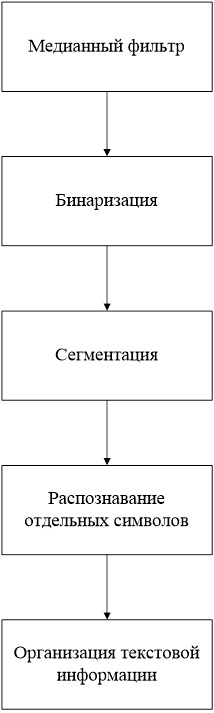
\includegraphics[scale=0.6]{Img01.jpg}}
\caption{Алгоритм распознавания текста}
\end{figure}


	      \addcontentsline{toc}{section}{  3.2 Медианный фильтр}
                  \section*{\normalsize\hspace{4ex} 3.2 Медианный фильтр}

   \hspace{4ex} Множество изображений полученных при съемке подвергаются импульсным помехам. При их воздействии на изображение, наблюдаются белые или черные точки, хаотически разбросанные по кадру.\
   
   \hspace{4ex} Данный фильтр применятся для минимизации шума и смазывания острых краев букв.\
   
   \hspace{4ex} При медианной фильтрации используется двумерное окно обычно имеющее центральную симметрию, при этом его центр располагается в текущей точке фильтрации. На рисунке 2 показаны два примера наиболее часто применяемых вариантов окон в виде креста и в виде квадрата[3].\

\begin{figure}[h!]
\center{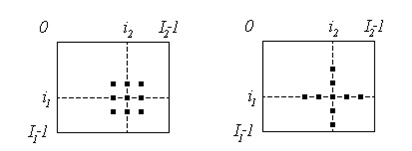
\includegraphics{Img02.jpg}}
\caption{Примеры окон при медианной фильтрации}
\end{figure}

   \hspace{4ex}Значения отсчётов внутри окна фильтра сортируются в порядке возрастания (убывания); и значение, находящееся в середине упорядоченного списка, поступает на выход фильтра. Окно перемещается вдоль фильтруемого сигнала и вычисления повторяются[2].\
  

                 \addcontentsline{toc}{section}{ 3.3 Обработка исключительных ситуаций}
                  \section*{\normalsize\hspace{4ex}3.3 Обработка исключительных ситуаций}

\hspace{4ex} Бинаризация изображений, т.е. перевод полноцветного или в градациях серого изображения в монохромное, где присутствуют только два типа пикселей (темные и светлые) имеет большое значение при распознавании образов. Особенно это относится к бинарным объектам, таким, как штриховые коды, текст, чертежи и т.п. Существуют различные подходы к бинаризации, которые условно можно разделить на 2 группы:пороговые и адаптивные\

  \hspace {4ex}  В рамках моей курсовой работы будет рассмотрен только пороговый метод.
Пороговые методы бинаризации работают со всем изображением, находя какую-то характеристику (порог), позволяющую разделить все изображение на чёрное и белое. То есть все пиксели, значения которых меньше порога, становятся черными, а пиксели, значение которых выше порога, становятся белыми [7]. Данное действие реализуется функцией Monochrome.
\
  \hspace {4ex}  Существует множество методов вычисления порога бинаризации, однако, для упрощения алгоритма, порогу было присвоено константное значение.\

                   \addcontentsline{toc}{section}{ 3.4 Сегментация}
                  \section*{\normalsize\hspace{4ex}3.4 Сегментация}
  \hspace {4ex} Для процесса сегментации принята следующая эвристика. Предполагается, что предложения текста расположены горизонтально и не создают пересечений друг с другом. Поэтому алгоритм нахождения поисковых узоров можно разделить на следующие этапы:\
  
  \hspace {4ex} 1) GetMatrix – Преобразование изображения в двумерный массив единиц (пиксели черного цвета) и нулей (пиксели белого цвета);\
  
  \hspace {4ex} 2) FindSymbols  – Сканирование элементов матрицы, с целью поиска единичного значения;\
  
  \hspace {4ex} 3) AbsorbSymbol – Если единица была найдена, то, используя алгоритм поиска в глубину, вырезаем множество смежных единиц, заменяя их значения нулями, чтобы исключить возможность повторного считывания. Во время данного процесса вычисляются и сохраняются такие значения, как верхняя, нижняя, правая, левая границы символа;\
  
  \hspace {4ex} 4) CutSymbol – После полного исследования матрицы, на выходе имеем массив элементов хранящих границы символов, которые были расположены на изображении. Используя полученные значения, вырезаем символы из преобразованного фильтрами изображения;\
  
  \hspace {4ex} 5) LeadToThePattern  – Приведение размеров изображений символов к размерам обучающих шаблонов.\
  
  					 \addcontentsline{toc}{section}{ 3.5 Нейронные сети Кохонена}
                  \section*{\normalsize\hspace{4ex}3.5 Нейронные сети Кохонена} 
                   
                   \addcontentsline{toc}{section}{ 3.5.1 Структура сети}
                  \section*{\normalsize\hspace{4ex}3.5.1 Структура сети}
                  
  \hspace {4ex} Для применения нейронных сетей Кохонена в задачах классификации требуется некоторая формализация. Каждый объект, который требуется классифицировать, представляется в виде некоторого вектора, подающегося на вход нейронной сети. В программе этот вектор представлен одномерным массивов состоящим из нулей и единиц. Составленние массива происходит при построчном сканировании изображения символа, приведенного к нужному размеру. Нулевые и единичные значение присваиваются в соответствии с цветом сканируемого пикселя(черный - единица, белый - ноль) [6].\
  
  \hspace {4ex} Количество нейронов во входном слое определяется количеством компонентов этого входного вектора. Количество же выходов определяется количеством классов, т.е. если необходимо определить к какой букве алфавита относится входной вектор, то количество нейронов в выходном слое будет равно размеру алфавита выбранного языка. Таким образом, каждый нейрон в выходном слое «отвечает» за свою букву. Значения, которые принимают нейроны в выходном слое, отображают насколько вектор классифицируемого символа на входе близок, по мнению нейронной сети Кохонена, к тому или иному классу. Чем больше «уверенность», что объект принадлежит к тому или иному классу, тем больше значение принимает нейрон соответствующего класса.\
  
  \begin{figure}[h!]
\center{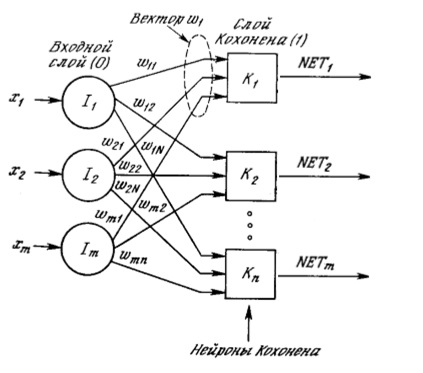
\includegraphics{Img03.jpg}}
\caption{Нейронная сеть Кохонена}
\end{figure}
  
  \hspace {4ex} Каждый нейрон выходного слоя может принимать значение либо ноль, либо единица. При этом для одного входного вектора единице может быть равен один и только один нейрон выходного слоя, т.е. один объект не может относиться сразу к двум классам. 
Рассмотрим следующую нейронную сеть Кохонена с m входами и n выходами, т.е. нейронную сеть для классификации по n классам:\

  
  \hspace {4ex} На рисунке 3 нейрон Кохонена K1 имеет веса w11, w21, …, wm1, составляющие весовой вектор W1. Они соединяются через входной слой с входными сигналами x1, x2, …, xm, составляющими входной вектор X. Подобно нейронам большинства сетей выход NET каждого нейрона Кохонена является просто суммой взвешенных входов.\
  
  \hspace {4ex} Нейрон Кохонена с максимальным значением NET является «победителем». Его выход равен единице, у остальных он равен нулю[1].В программе выходные значения  нейронов вычисляется при передаче классифицируемого вектора в функцию  Parse. Нейрон с наибольшим значением NET определяется в функции FindNeuronWithMaxExcitation. Чтобы сеть можно было использовать повторно, по завершению классификации, импульс каждого нейрона обнуляется при вызове метода SetZeroExcitations.


                      \addcontentsline{toc}{section}{ 3.5.2 Обучения слоя Кохонена}
                  \section*{\normalsize\hspace{4ex}3.5.2 Обучения слоя Кохонена}
  \hspace {4ex} Чтобы коэффициенты входов были правильно настроены, необходимо сначала обучить сеть. Как правило, обучающее множество включает много сходных между собой входных векторов, и сеть должна быть обучена активировать один и тот же нейрон Кохонена для каждого из них. В этом случае веса этого нейрона должны получаться усреднением входных векторов, которые должны его активировать. Этим занимается отдельный модуль обучения. Данный модуль берет очередное изображение из обучающей выборки и указывает сети к какому классу оно относиться. Сеть анализирует все позиции черных пикселей и выравнивает коэффициенты нейрона отвечающего за указанный класс, минимизируя ошибку совпадения.\
  
  \begin{figure}[h!]
\center{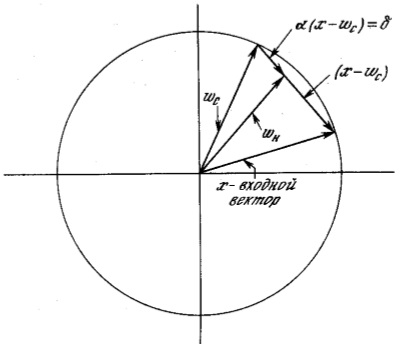
\includegraphics{Img04.jpg}}
\caption{Вращение весового вектора в процессе обучения
(Wн – вектор новых весовых коэффициентов, Wc – вектор старых весовых коэффициентов)}
\end{figure}
 
  \hspace {4ex} Переменная a является коэффициентом скорости обучения, который вначале  равен 0,7 и постепенно уменьшаться в процессе обучения, при каждом вызове метода Study. Постепенное уменьшение величины a уменьшает воздействие каждого обучающего шага, так что окончательное значение будет средней величиной от входных векторов, на которых происходит обучение.\   
  \begin{figure}[h!]
\center{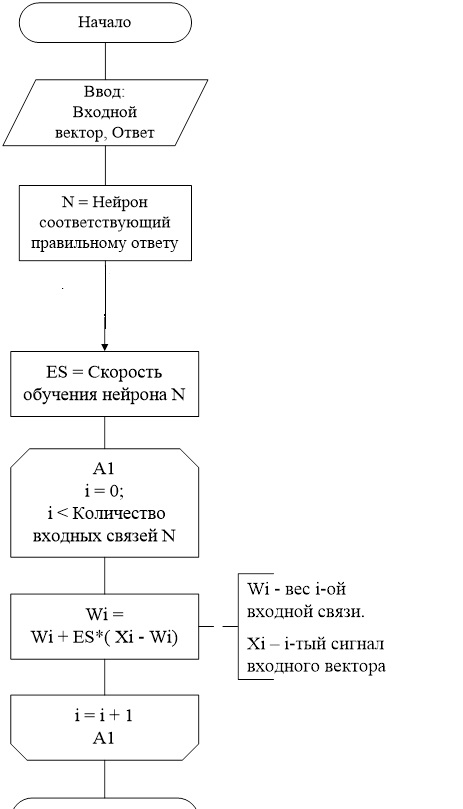
\includegraphics{Img05.jpg}}
\caption{Алгоритм выравнивания весовых коэффициентов}
\end{figure}  

			\addcontentsline{toc}{section}{ 3.5.3 Предварительная обработка входных векторов}
            \section*{\normalsize\hspace{4ex}3.5.3 Предварительная обработка входных векторов}           
   \hspace {4ex} Весьма желательно нормализовать входные векторы перед тем, как предъявлять их сети. Это выполняется с помощью деления каждой компоненты входного вектора на длину вектора. Эта длина находится извлечением квадратного корня из суммы квадратов компонент вектора. \
   
   \hspace {4ex} Это превращает входной вектор в единичный вектор с тем же самым направлением, т. е. в вектор единичной длины в n-мерном пространстве. Данное действие реализуется функцией NormaizeVector.\
   
   \begin{figure}[h!]
\center{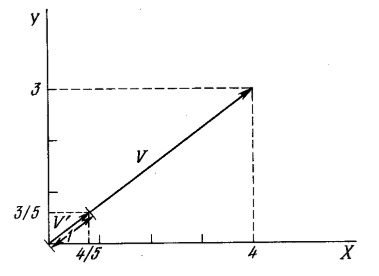
\includegraphics{Img06.jpg}}
\caption{Единичный входной вектор}
\end{figure}
   
   \addcontentsline{toc}{section}{ 3.5.4 Выбор начальных значений весовых векторов}
            \section*{\normalsize\hspace{4ex}3.5.4 Выбор начальных значений весовых векторов}
            
   \hspace {4ex} Одно из решений, известное под названием метода выпуклой комбинации (convex combination method), состоит в том, что все веса приравниваются одной и той же величине.\       
   
   \hspace {4ex} Вначале a очень мало, вследствие чего все входные векторы имеют длину, близкую к 1/n , и почти совпадают с векторами весов. В процессе обучения сети a постепенно возрастает, приближаясь к единице. Это позволяет разделять входные векторы и окончательно приписывает им их истинные значения[1].\ 
   
   \hspace {4ex} Уменьшение резкости возрастания a, при не достаточном числе обучающих выборок, может быть достигнуто путем увеличения обучающих процессов по выборкам. В программе, при каждом вызове метода Study, значение a увеличивается на такое значение сигма, что к концу процесса обучения сети, a принимает значение близкое к единице.
Нормализация обучающих векторов реализована в функции  NormaizeStudyVector.\

 				\addcontentsline{toc}{section}{ 3.6 Организация текстовой информации}
                  \section*{\normalsize\hspace{4ex}3.6 Организация текстовой информации} 
                  
       \addcontentsline{toc}{section}{ 3.6.1 Пространственное расположение}
            \section*{\normalsize\hspace{4ex}3.6.1 Пространственное расположение} 
                     
 \hspace {4ex} При помощи нейронной сети Кохонена входные символы были распределены по классам, однако в разделенном состоянии они не несут никакой информационной нагрузки. Поэтому необходимо составить текст в соответствии с расположением символов на обрабатываемом изображении. \     
 
 \hspace {4ex} В процессе сегментации для каждого вырезанного символа были сохранены его границы. Используя эти значения можно найти координаты центра символа на исходном изображении следующим образом:

\hspace {4ex} x = (Right + Left)/2;
\hspace {4ex} y = (Bottom + Top)/2;

\hspace {4ex} Символы в списке сортируются по их пространственному расположению слева направо, сверху вниз[5].

\begin{figure}[h!]
\center{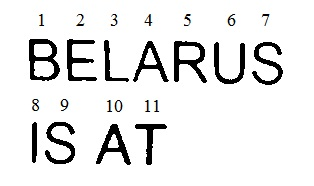
\includegraphics{Img07.jpg}}
\caption{Пример нумерации символов}
\end{figure}

 			\addcontentsline{toc}{section}{ 3.6.2 Переходы к новой строке}
            \section*{\normalsize\hspace{4ex}3.6.2 Переходы к новой строке}
            
\hspace {4ex} Так как предполагается, что предложения текста расположены горизонтально и не создают пересечений друг с другом. То, для того, чтобы определить переход к новой строке, можно использовать следующий алгоритм:\
            
\begin{figure}[h!]
\center{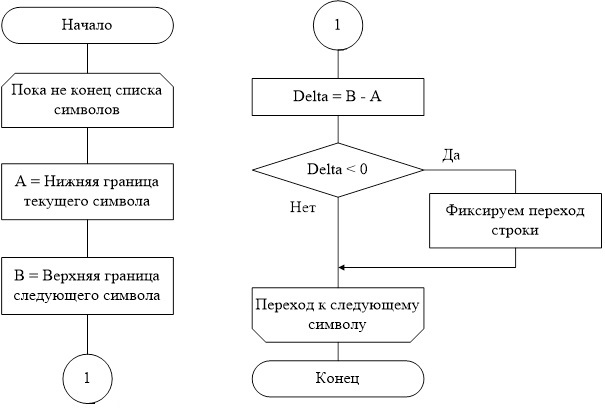
\includegraphics{Img08.jpg}}
\caption{Алгоритм определения переходов к новой строке}
\end{figure} 

\addcontentsline{toc}{section}{ 3.6.3 Поиск пробелов}
            \section*{\normalsize\hspace{4ex}3.6.3 Поиск пробелов}

\hspace {4ex} Поиск пробелов в строке текста на удивление сложная задача. Хотя у человека при чтении текста даже на неизвестном языке практически никогда не возникает проблемы найти пробелы в тексте, при автоматической классификации все время возникают разные проблемы.
\hspace {4ex} Базовая идея заключается в следующем – ищутся на изображении строки вертикальные белые просветы, а дальше классифицируются по ширине: широкие просветы – это пробелы между словами, узкие – между символами[4].
            
 \begin{figure}[h!]
\center{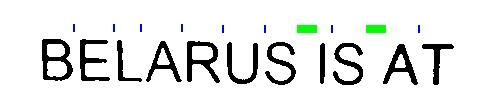
\includegraphics{Img09.jpg}}
\caption{Пример вертикальных просветов}
\end{figure}

\hspace {4ex} Идея замечательная, но в реальной жизни ширина пробелов может быть очень неоднозначным показателем.

%-----5 ПРИМЕР РАБОТЫ------
	\newpage
	\addcontentsline{toc}{section}{5 ПРИМЕР РАБОТЫ}
           \section*{\normalsize\hspace{4ex}5 ПРИМЕР РАБОТЫ}

\hspace {4ex} 1)	Загрузка исходного изображения;

 \begin{figure}[h!]
\center{
\includegraphics{Img10.jpg}}
\caption{Исходное изображение}
\end{figure}

\hspace {4ex} 2)	Медианная фильтрация изображения;

 \begin{figure}[h!]
\center{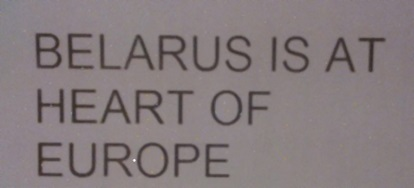
\includegraphics{Img11.jpg}}
\caption{Результат применения медианного фильтра}
\end{figure}

\hspace {4ex} 3)	Бинаризация изображения;

 \begin{figure}[h!]
\center{
\includegraphics{Img12.jpg}}
\caption{Результат бинаризации изображения}
\end{figure}

\hspace {4ex} 4)	Сегментация;

 \begin{figure}[h!]
\center{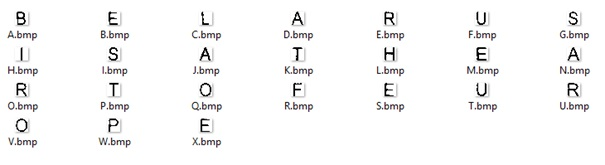
\includegraphics{Img13.jpg}}
\caption{Результат сегментации}
\end{figure}



\hspace {4ex} 5)	Распознавание и организация текстовой информации;

 \begin{figure}[h!]
\center{
\includegraphics{Img14.jpg}}
\caption{Результат распознавания}
\end{figure}  

\hspace {4ex}В результате распознавания были допущены две ошибки. Данное отклонение обусловлено не достаточным количеством и качеством обучающих выборок созданных для обучения нейронной сети. А так же на основе этого можно утверждать о том, что качественное распознавание не возможно при использовании единственного классификатора – нейронной сети Кохонена.\
         
 	
 	
	%-------ЗАКЛЮЧЕНИЕ-------
	\newpage
	\addcontentsline{toc}{section}{ЗАКЛЮЧЕНИЕ}
	\section*{\center\normalsize ЗАКЛЮЧЕНИЕ \endcenter}
	\hspace{4ex}В результате работы была создана программа, позволяющая распознавать текстовую информацию. \

	\hspace{4ex}Созданная программа позволяет пользователю, распознавать текст, при использовании изображений высокого либо среднего качества, со слабым шумом либо без него.\

\hspace{4ex}В качестве направления для дальнейшей работы с программой распознавания  можно выделить:\

\hspace{4ex} 1)Выбор более сложных иерархических моделей нейросетей организованных аналогично зрительной коре (Когнитрон, Неокогнитрон).

\hspace{4ex} 2)Комбинированное использование стандартных классификаторов




	%----СПИСОК ИСПОЛЬЗОВАННОЙ ЛИТЕРАТУРЫ-------
	\newpage
	\addcontentsline{toc}{section}{СПИСОК ИСПОЛЬЗОВАННОЙ ЛИТЕРАТУРЫ}
	\section*{\center\normalsize СПИСОК ИСПОЛЬЗОВАННОЙ ЛИТЕРАТУРЫ \endcenter}

\hspace{4ex}[1] Уоссермен, Ф. Нейрокомпьютерная техника:  Теория и практика: пер. с англ. Ю. А. Зуев / В. А. Точенов – М. : Феникс, 1992. – 184 с.\
 
\hspace{4ex}[2] Научная библиотека избранных естественно-научных изданий [Электронный ресурс]. – Электронные данные. – Режим доступа: http://sernam.ru/book_kir.php?id=25.\

\hspace{4ex}[3] Цифровая обработка изображений [Электронный ресурс]. – Электронные данные. – Режим доступа: http://www.sibsauktf.ru/courses/fulleren/g3.htm.\

\hspace{4ex}[4] Распознавание текста в ABBYY FineReader [Электронный ресурс]. – Электронные данные. – Режим доступа: http://habrahabr.ru/company/abbyy/blog/225215.\

\hspace{4ex}[5] Методы распознавания текста [Электронный ресурс]. – Электронные данные. – Режим доступа: http://habrahabr.ru/post/220077.\

\hspace{4ex}[6]Нейронные сети [Электронный ресурс]. – Электронные данные. – Режим доступа: http://www.aiportal.ru/articles/neural-networks/1/.\

\hspace{4ex}[7] Бинаризация изображений а [Электронный ресурс]. – Электронные данные. – Режим доступа: http://recog.ru/blog/applied/15.html.\






	%----ПРИЛОЖЕНИЕ А (обязательное) Исходный код программы----
	
	\newpage
	\addcontentsline{toc}{section}{ПРИЛОЖЕНИЕ А}
	\section*{\center\normalsize ПРИЛОЖЕНИЕ А\\(обязательное)\\Исходный код программы \endcenter}
	
	\begin{verbatim}
	class Program
{
        static void Main(string[] args)
        {
            var bmp = new Bitmap(
Bitmap.FromFile(@"C:\Users\Andrew\Desktop\belphoto.jpg")
     );

            var kn = new KohonenNetwork();
            var td = new TextDetector();
            var recognizer = new Recognizer(kn, td);
            var Message = recognizer.Parse(bmp);

            Console.WriteLine(Message);
        }
}

class Neuron
{
        public Link[] IncomingLinks;
        public double Power { get; set; }
        private double _es = 0.79;
        private double _alpha = 0.001;
        public double Alpha { get { _alpha *= 1.28; return _alpha; } }
        public double EducationSpeed { get { _es *= 0.9; return _es; } }

        public Neuron(int LinksCount)
        {
            IncomingLinks = new Link[LinksCount];
            Power = 0;
        }
}


class Link
{
        public Neuron Neuron;
        public double Weight;

        public Link(Neuron neuron)
        {
            Neuron = neuron;
            Weight = 0;
        }
}


class Input
{
        public Link[] OutgoingLinks;

        public Input(int LinksCount)
        {
            OutgoingLinks = new Link[LinksCount];
        }
}


class KohonenNetwork
{
        private readonly Input[] _inputs;
        private readonly Neuron[] _neurons;
        public static readonly int _alphabetLen = 26;
        private readonly int _pixelsNumber;

        public KohonenNetwork()
        {
            _pixelsNumber = 16 * 16;
            _inputs = new Input[_pixelsNumber];
            _neurons = new Neuron[_alphabetLen];
            FieldInputs();
            FieldNeurons();
            CreateNetwork();
            SetZeroExcitations();
        }

        private void FieldInputs()
        {
            for (var i = 0; i < _pixelsNumber; i++)
                _inputs[i] = new Input(_alphabetLen);
        }

        private void FieldNeurons()
        {
            for (var i = 0; i < _alphabetLen; i++)
                _neurons[i] = new Neuron(_pixelsNumber);
        }

        private void CreateNetwork()
        {
            for (var j = 0; j < _pixelsNumber; j++)
            {
                for (var i = 0; i < _alphabetLen; i++)
                {
                    var link = new Link(_neurons[i]);
                    link.Weight = 1 / Math.Sqrt(_pixelsNumber);
                    _inputs[j].OutgoingLinks[i] = link;
                    _neurons[i].IncomingLinks[j] = link;
                }
            }
        }

        public int  Parse(int[] input)
        {
            var normalizedVector = Mat.NormaizeVector(input);
            for (var i = 0; i < _inputs.Length; i++)
            {
                var inputNeuron = _inputs[i];
                foreach (var outgoingLink in inputNeuron.OutgoingLinks)
                {
                    outgoingLink.Neuron.Power += outgoingLink.Weight * normalizedVector[i];
                }
            }
            var maxIndex = FindNeuronWithMaxExcitation();
            SetZeroExcitations();

            return maxIndex;
        }

        private int FindNeuronWithMaxExcitation()
        {
            var maxIndex = 0;
            for (var i = 1; i < _neurons.Length; i++)
            {
                if (_neurons[i].Power > _neurons[maxIndex].Power)
                    maxIndex = i;
            }
            return maxIndex;
        }

        private void SetZeroExcitations()
        {
            foreach (var outputNeuron in _neurons)
            {
                outputNeuron.Power = 0;
            }
        }

        public void Study(int[] input, int correctAnswer)
        {
            var neuron = _neurons[correctAnswer];
            var educationSpeed = neuron.EducationSpeed;
            var alpha = neuron.Alpha;
            var normalizedVector = NormaizeStudyVector(input, alpha);

            for (var i = 0; i < neuron.IncomingLinks.Length; i++)
            {
                var incomingLink = neuron.IncomingLinks[i];
                incomingLink.Weight = incomingLink.Weight + educationSpeed * (normalizedVector[i] - incomingLink.Weight);

            }
        }

        private double[] NormaizeStudyVector(int[] input, double alpha)
        {
            double[] normalizedVector = new double[input.Length];
            int n = input.Length;

            for (var i = 0; i < input.Length; i++)
            {
                normalizedVector[i] = alpha * input[i] + (1 - alpha) / Math.Sqrt(n);
            }
            return normalizedVector;
        }
}


class Filter
{
        public static void Median3x3(ref Bitmap image)
        {
            int[] dx = {0, 1, 1, 0, -1, -1, 1, -1, 0};
            int[] dy = {1, 0, 1, -1, 0, 1, -1, -1, 0};
            var arrR = new int[9];
            var arrG = new int[9];
            var arrB = new int[9];
            var outImage = new Bitmap(image);

            for (int i = 1; i < image.Width - 1; i++)
                for (int j = 1; j < image.Height - 1; j++)
                {
                    for (int i1 = 0; i1 < 9; i1++)
                    {
                        var point = image.GetPixel(i + dx[i1], j + dy[i1]);

                        arrR[i1] = point.R;
                        arrG[i1] = point.G;
                        arrB[i1] = point.B;
                    }
                    Array.Sort(arrR);
                    Array.Sort(arrG);
                    Array.Sort(arrB);

                    outImage.SetPixel(i, j, Color.FromArgb(arrR[4], arrG[4], arrB[4]));
                }

            image = outImage;
        }

        public static void Monochrome(ref Bitmap image, int level)
        {
            for (int j = 0; j < image.Height; j++)
            {
                for (int i = 0; i < image.Width; i++)
                {
                    var color = image.GetPixel(i, j);
                    int sr = (color.R + color.G + color.B) / 3;
                    image.SetPixel(i, j, (sr < level ? Color.Black : Color.White));
                }
            }
        }
}


class Symbol
{
        private int _x;
        private int _y;
        private int _top = int.MaxValue;
        private int _buttom = 0;
        private int _left = int.MaxValue;
        private int _right = 0;
        public bool isEmpty = true;

        public int CenterX { get { return _x; } }
        public int CenterY { get { return _y; } }
        public int Width { get { return _right - _left; } }
        public int Height { get { return _buttom - _top; } }
        public int Top { get { return _top; } }
        public int Buttom { get { return _buttom; } }
        public int Left { get { return _left; } }
        public int Rigt { get { return _right; } }

        public Bitmap Pattern { get; set; }

        public Symbol(){}

        public int[] GetVector()
        {
            return Mat.GetVector(Pattern);
        }

        private Bitmap LeadToThePattern(Bitmap image)
        {
            if (image.Height < 5 && image.Width < 5)
                return new Bitmap(16, 16);
            
            int newWidth = 16;
            int newHeight = 16;

            if (image.Height > image.Width)
                newWidth = (int)(image.Width / ((float)image.Height / 16));
            
            if (image.Height < image.Width)
                newHeight = (int)(image.Height / ((float)image.Width / 16));

            Bitmap newImage = new Bitmap(image, new Size(newWidth, newHeight));

            Bitmap tmpFile = new Bitmap(16, 16);
            Graphics gr = Graphics.FromImage(tmpFile);
            gr.Clear(Color.White);
            gr.DrawImage(newImage, new Point((16 - newWidth) / 2, 0));

            return tmpFile;
        }

        public void CutSymbol(ref Bitmap image)
        {
            RectangleF cloneRect = new RectangleF(_left, _top, _right - _left + 2, _buttom - _top + 2);
            System.Drawing.Imaging.PixelFormat format =
                image.PixelFormat;
            Bitmap cloneBitmap = image.Clone(cloneRect, format);

            var img = LeadToThePattern(cloneBitmap);
            Filter.Monochrome(ref img, 200);
            Pattern = img;
        }

        public void AddBlackPoint(int x, int y)
        {
            if (y > _buttom)
                _buttom = y;
            if (y < _top)
                _top = y;
            if (x < _left)
                _left = x;
            if (x > _right)
                _right = x;
            isEmpty = false;
            CountCenter();
        }

        private void CountCenter()
        {
            _x = (_left + _right) / 2;
            _y = (_top + _buttom) / 2;
        }
}


class TextDetector
{
        private Bitmap _image;
        private int[][] _matrix;
        private List<Symbol> _symbols;

        private int[] dx = {0, 1, 1, 0, -1, -1, 1, -1};
        private int[] dy = {1, 0, 1, -1, 0, 1, -1, -1};

        public List<Symbol> Symbols { get { return _symbols; } }

        public TextDetector() { }

        public void Detect(Bitmap image)
        {
            _image = image;
            _symbols = new List<Symbol>();
            _matrix = Mat.GetMatrix(_image);
            FindSymbols();
            SortSymbols();
        }

        public List<int[]> GetVectors()
        {
            List<int[]> vectors = new List<int[]>();
            for (int i = 0; i < _symbols.Count; i++)
                vectors.Add(_symbols[i].GetVector());

            CompleteTextOrganization(vectors);

            return vectors;
        }

        public void CompleteTextOrganization(List<int[]> vectors)
        {
            var enterVector = Mat.GetEnterVector();
            var spaceVector = Mat.GetSpaceVector();
            var deltaI = 0;

            int[] spaces = FindSpaces();
            int[] enters = FindLineCompletions();

            for (var i = 1; i < _symbols.Count; i++)
            {
                if (spaces[i] == 1)
                {
                    vectors.Insert(i + deltaI, spaceVector);
                    deltaI++;
                }

                if (enters[i] == 1)
                {
                    vectors.Insert(i + deltaI, enterVector);
                    deltaI++;
                }
            }
        }

        private int[] FindLineCompletions()
        {
            var result = new int[_symbols.Count];
            var deltaY = 0;

            for (int i = 1; i < _symbols.Count; i++)
            {
                deltaY = (_symbols[i - 1].Buttom - _symbols[i].Top);
                if (deltaY < 0)
                    result[i] = 1;
                else
                    result[i] = 0;
            }

            return result;
        }

        private int[] FindSpaces()
        {
            var result = new int[_symbols.Count];
            var spaces = new List<int>(){-1};
            var deltaY = 0;
            var deltaX = 0;
            for (var i = 1; i < _symbols.Count; i++)
            {
                deltaY = (_symbols[i - 1].Buttom - _symbols[i].Top);
                deltaX = _symbols[i].Left - _symbols[i - 1].Rigt;
                if (deltaY > 0)
                    spaces.Add(deltaX);
                else
                    spaces.Add(-1);
            }
            double avSpaceWidth = spaces.Max() / 2;

            for (var i = 1; i < _symbols.Count; i++)
            {
                deltaY = (_symbols[i - 1].Buttom - _symbols[i].Top);
                if (spaces[i] > avSpaceWidth && deltaY > 0)
                    result[i] = 1;
                else
                    result[i] = 0;
            }

            return result;
        }

        private void SortSymbols()
        {
            _symbols.Sort(delegate(Symbol x, Symbol y)
            {
                if (x.CenterY - y.CenterY > 10) return 1;
                if (x.CenterY - y.CenterY < -10) return -1;
                if (x.CenterX >= y.CenterX) return 1;
                if (x.CenterX < y.CenterX) return -1;
                    return 0;
            }
            );
        }

        private void FindSymbols()
        {
            Symbol newSymbol;
            for (int i = 0; i < _image.Height; i++)
                for (int j = 0; j < _image.Width; j++)
                    if (_matrix[i][j] == 1)
                    {
                        newSymbol  = new Symbol();
                        AbsorbSymbol(j, i, newSymbol);
                        if (!newSymbol.isEmpty)
                        _symbols.Add(newSymbol);
                    }
            CutSymblos();
        }

        private void AbsorbSymbol(int x, int y, Symbol symbol)
        {
            if (x < 0 || x >= _image.Width || y < 0 || y > _image.Height)
                return;
            if (_matrix[y][x] == 0)
                return;

            symbol.AddBlackPoint(x, y);
            _matrix[y][x] = 0;
            for (int i = 0; i < 8; i++)
                for (int j = 0; j < 8; j++)
                    AbsorbSymbol(x + dx[i], y + dy[j], symbol);
        }

        private void CutSymblos()
        {
            foreach (var symbol in _symbols)
                symbol.CutSymbol(ref _image);
        }
}


static class Mat
{
        static public int[][] GetMatrix(Bitmap image)
        {
            int[][] matrix = new int[image.Height][];
            for (var i = 0; i < image.Height; i++)
            {
                matrix[i] = new int[image.Width];
                for (var j = 0; j < image.Width; j++)
                    if (isBlack(image.GetPixel(j, i)))
                        matrix[i][j] = 1;
                    else
                        matrix[i][j] = 0;
            }

            return matrix;
        }

        static public int[] GetVector(Bitmap image)
        {
            var vector = new int[16 * 16];
            for (var i = 0; i < 16; i++)
                for (var j = 0; j < 16; j++)
                    if (isBlack(image.GetPixel(j, i)))
                        vector[i * 16 + j] = 1;
                    else
                        vector[i * 16 + j] = 0;

            return vector;
        }

        
        static public int[] GetEnterVector()
        {
            return new int[1];
        }

        static public int[] GetSpaceVector()
        {
            return new int[2];
        }

        static public bool isSpaceVector(int[] vector)
        {
            return vector.Length == 2;
        }

        static public bool isEnterVector(int[] vector)
        {
            return vector.Length == 1;
        }

        static public bool isBlack(Color color)
        {
            if (color.R == 0 && color.G == 0 && color.B == 0)
                return true;
            else
                return false;
        }

        static public double CalculateVectorLength(int[] input)
        {
            double sumOfSquares = 0;
            for (var i = 0; i < input.Length; i++)
            {
                sumOfSquares += input[i] * input[i];
            }

            return Math.Sqrt(sumOfSquares);
        }

        static public double CalculateVectorLength(double[] input)
        {
            double sumOfSquares = 0;
            for (var i = 0; i < input.Length; i++)
            {
                sumOfSquares += input[i] * input[i];
            }

            return Math.Sqrt(sumOfSquares);
        }

        static public double[] NormaizeVector(int[] input)
        {
            double[] normalizedVector = new double[input.Length];
            var vectorLength = CalculateVectorLength(input);

            for (var i = 0; i < input.Length; i++)
            {
                normalizedVector[i] = input[i] / vectorLength;
            }
            return normalizedVector;
        }
}


class Recognizer
{
        private KohonenNetwork _kn;
        private TextDetector _td;

        private double[][] _matchingPercents;

        public Recognizer(KohonenNetwork kn, TextDetector td)
        {
            _kn = kn;
            _td = td;
            StudyNetwork();
        }

        public List<Symbol> GetSymbols()
        {
            return _td.Symbols;
        }

        public double[][] GetMatchingPercents()
        {
            return _matchingPercents;
        }

        public string Parse(Bitmap image)
        {
            Filter.Median3x3(ref image);
            Filter.Monochrome(ref image, 100);
            
            _td.Detect(image);
            var vectros = _td.GetVectors();
            var message = String.Empty;

            int i = 0;
            foreach (var vector in vectros)
                if (Mat.isSpaceVector(vector))
                    message += ' ';
                else if (Mat.isEnterVector(vector))
                    message += '\n';
                else
                {
                    message += (char)(_kn.Parse(vector) + 'A');
                    _matchingPercents[i++] = _kn.MatchingPercents;
                }

            return message;
        }

        private void StudyNetwork()
        {
            for (var i = 0; i < 10; i++)
            {
                LearnFont("Arial16x16(photo)changed");
                LearnFont("Arial16x16(50)");
                LearnFont("Arial16x16photo");
                LearnFont("Arial16x16(photo)");
                LearnFont("Arial16x16");
            }
        }

        private void LearnFont(string Font)
        {
            Bitmap bmp;
            int[] vector;
            char symbol;

            _kn._fonts++;

            for (var i = 0; i < 26; i++)
            {
                symbol = (char)('A' + i);
                bmp = new Bitmap(Bitmap.FromFile(@"C:\Users\Alexander\Desktop\"
                    + Font + @"\" + symbol + ".bmp"));
                vector = Mat.GetVector(bmp);
                _kn.Study(vector, i);
            }
        }

        public void SetKohonenNetwork(KohonenNetwork kn)
        {
            _kn = kn;
        }

        public void SetTextDetector(TextDetector td)
        {
            _td = td;
        }
 }

	\end{verbatim}
	
	
\end{document}          
